\chapter{System Architecture}\label{section:overview}

\section{Overview}
The Internet of Things (IoT) is a new technology that allows devices to connect remotely to achieve smart
farming \cite{agriculture12101745}. The IoT has a wide range of applications in agriculture, and it has 
began to influence many other industries as well, such as healthcare, transportation, and manufacturing. 
This was done to improve the efficiency and productivity of these industries, 
as well as to reduce costs and improve the quality of products and services\cite{s19081833}.

The PiIrrigate smart irrigation system is build using a combination of hardware and software technologies.
It leverages both low-power edge devices and cloud-based infrastructure to provide real-time monitoring
and data collection, as well as remote control capabilities.
The core components and their roles in the system are as follows:
\begin{itemize}
  \item \textbf{ESP32 (LILYGO Meshtastic AXP2101 T-Beam V1.2 ESP32 LoRa)} \\
  The LILYGO Meshtastic AXP2101 T-Beam V1.2 ESP32 LoRa is a development board based on the ESP32 microcontroller, it is equipped with
  LoRa radio communication capabilities, Wifi, Bluetooth, GPS, and a battery management system.
  It is used to collect data from sensors and send it to the gateway using LoRa radio communication.

  \item \textbf{Raspberry Pi} \\
  Raspberry Pi is a small, affordable computer that can be used for a wide range of applications.
  The Raspberry Pi is the core of the PiIrrigate irrigation module, 
  it is responsible for receiving data from the ESP32 nodes and sending it to Azure IoT Hub.

  \item \textbf{Azure IoT Hub} \\
  Azure IoT Hub is a cloud-based service that enables secure and reliable communication 
  between IoT devices and the cloud.
  It manages the bidirectional communication between the Raspberry Pi and the web API.

  \item \textbf{Web API} \\
  The web API is developed in .NET and is responsible for receiving data from the Raspberry Pi,
  storing it in a PostgreSQL database, and providing a way to access the data.
  SignalR is used to provide real-time communication between the server and the client.
  It also provides a way to control the system manually and to add new nodes to the system.

  \item \textbf{PostgreSQL Database} \\
  PostgreSQL is a powerful, open-source relational database management system.
  It is used to store the data collected from the sensors and the schedules sent to the system. It also
  stores the user data and the configuration of the system. The database is hosted in Neon.

  \item \textbf{Web Application} \\
  The web applicaiton is developed using Angular and is responsible for displaying live, historical data
  and provide the user interface for controlling the system.
\end{itemize}

In the following sections, we will explore each of these components in more detail,
starting with the hardware components and then moving on to the software components.

\section{Hardware Components}
\subsection{Sensors}
The PiIrrigate system uses a variety of sensors to collect data from the environment.
The sensors used in the PiIrrigate system are:
\begin{itemize}
  \item \textbf{Soil Moisture Sensor} \\
  The soil moisture sensor is used to measure the moisture level in the soil. It is used to determine when to irrigate the plants.

  \item \textbf{Temperature and Humidity Sensor} \\
  The temperature and humidity sensor is used to measure the temperature and humidity of the environment.
  It is used to determine the optimal conditions for plant growth and to adjust the irrigation schedule accordingly.

  \item \textbf{Rain Sensor} \\
  The rain sensor is used to detect rain and prevent irrigation during rainy weather. 
  It helps to conserve water and prevent over-irrigation.

  \item \textbf{Water Flow Sensor} \\
  The water flow sensor is used to measure the flow rate of water in the irrigation system.
  It is used to monitor the water consumption.

  \item \textbf{Water Temperature Sensor} \\
  The water temperature sensor is used to measure the temperature of the water in the irrigation system.
  It is used to ensure that the water temperature is within the optimal range for plant growth.

\end{itemize}
\subsection{ESP32 (LilyGo T-Beam)}

The T-Beam ESP32 LoRa Wireless Module is a compact development board thaht combines an ESP32 microcontroller,
LoRa transceiver (SX1278), GPS module, and a battery management system into a single unit. This board is ideal
for long-range, low-power IoT applications such as mesh networks, asset tracking, smart agriculture and environmental
monitoring. Besides this, it has a built-in OLED display. The communication range of the LoRa transceiver can reach up to 10 km in open areas.
\begin{figure}[H]
    \centering
    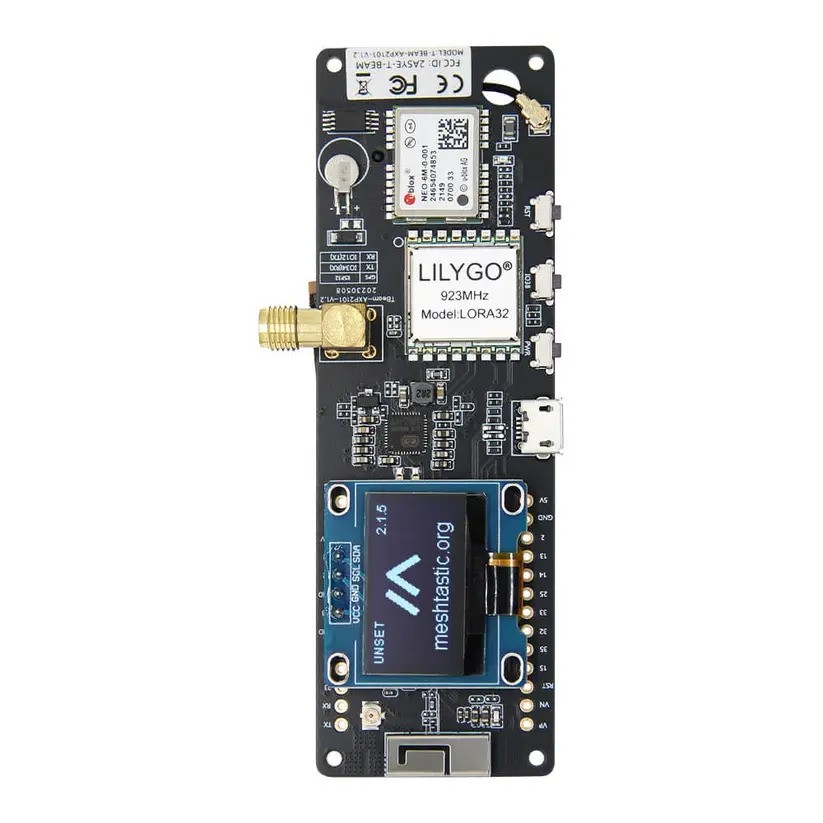
\includegraphics[width=0.5\textwidth]{images/esp32lora.jpg}
    \caption{ESP32 (LilyGo T-Beam) module used in PiIrrigate}
    \label{fig:esp32lora}
\end{figure}

\subsection{Raspberry Pi 4 Model B}
The Raspberry Pi 4 Model B is a small, affordable computer that can be used for a wide range of applications.
It is equipped with a quad-core ARM Cortex-A72 processor, up to 8GB of RAM, and supports dual-band Wi-Fi and Bluetooth.
The Raspberry Pi 4 Model B together with an ESP32LoRa is used in the PiIrrigate project as the gateway that receives data from the ESP32 nodes
and sends it to IoT Hub.
\begin{figure}[H]
    \centering
    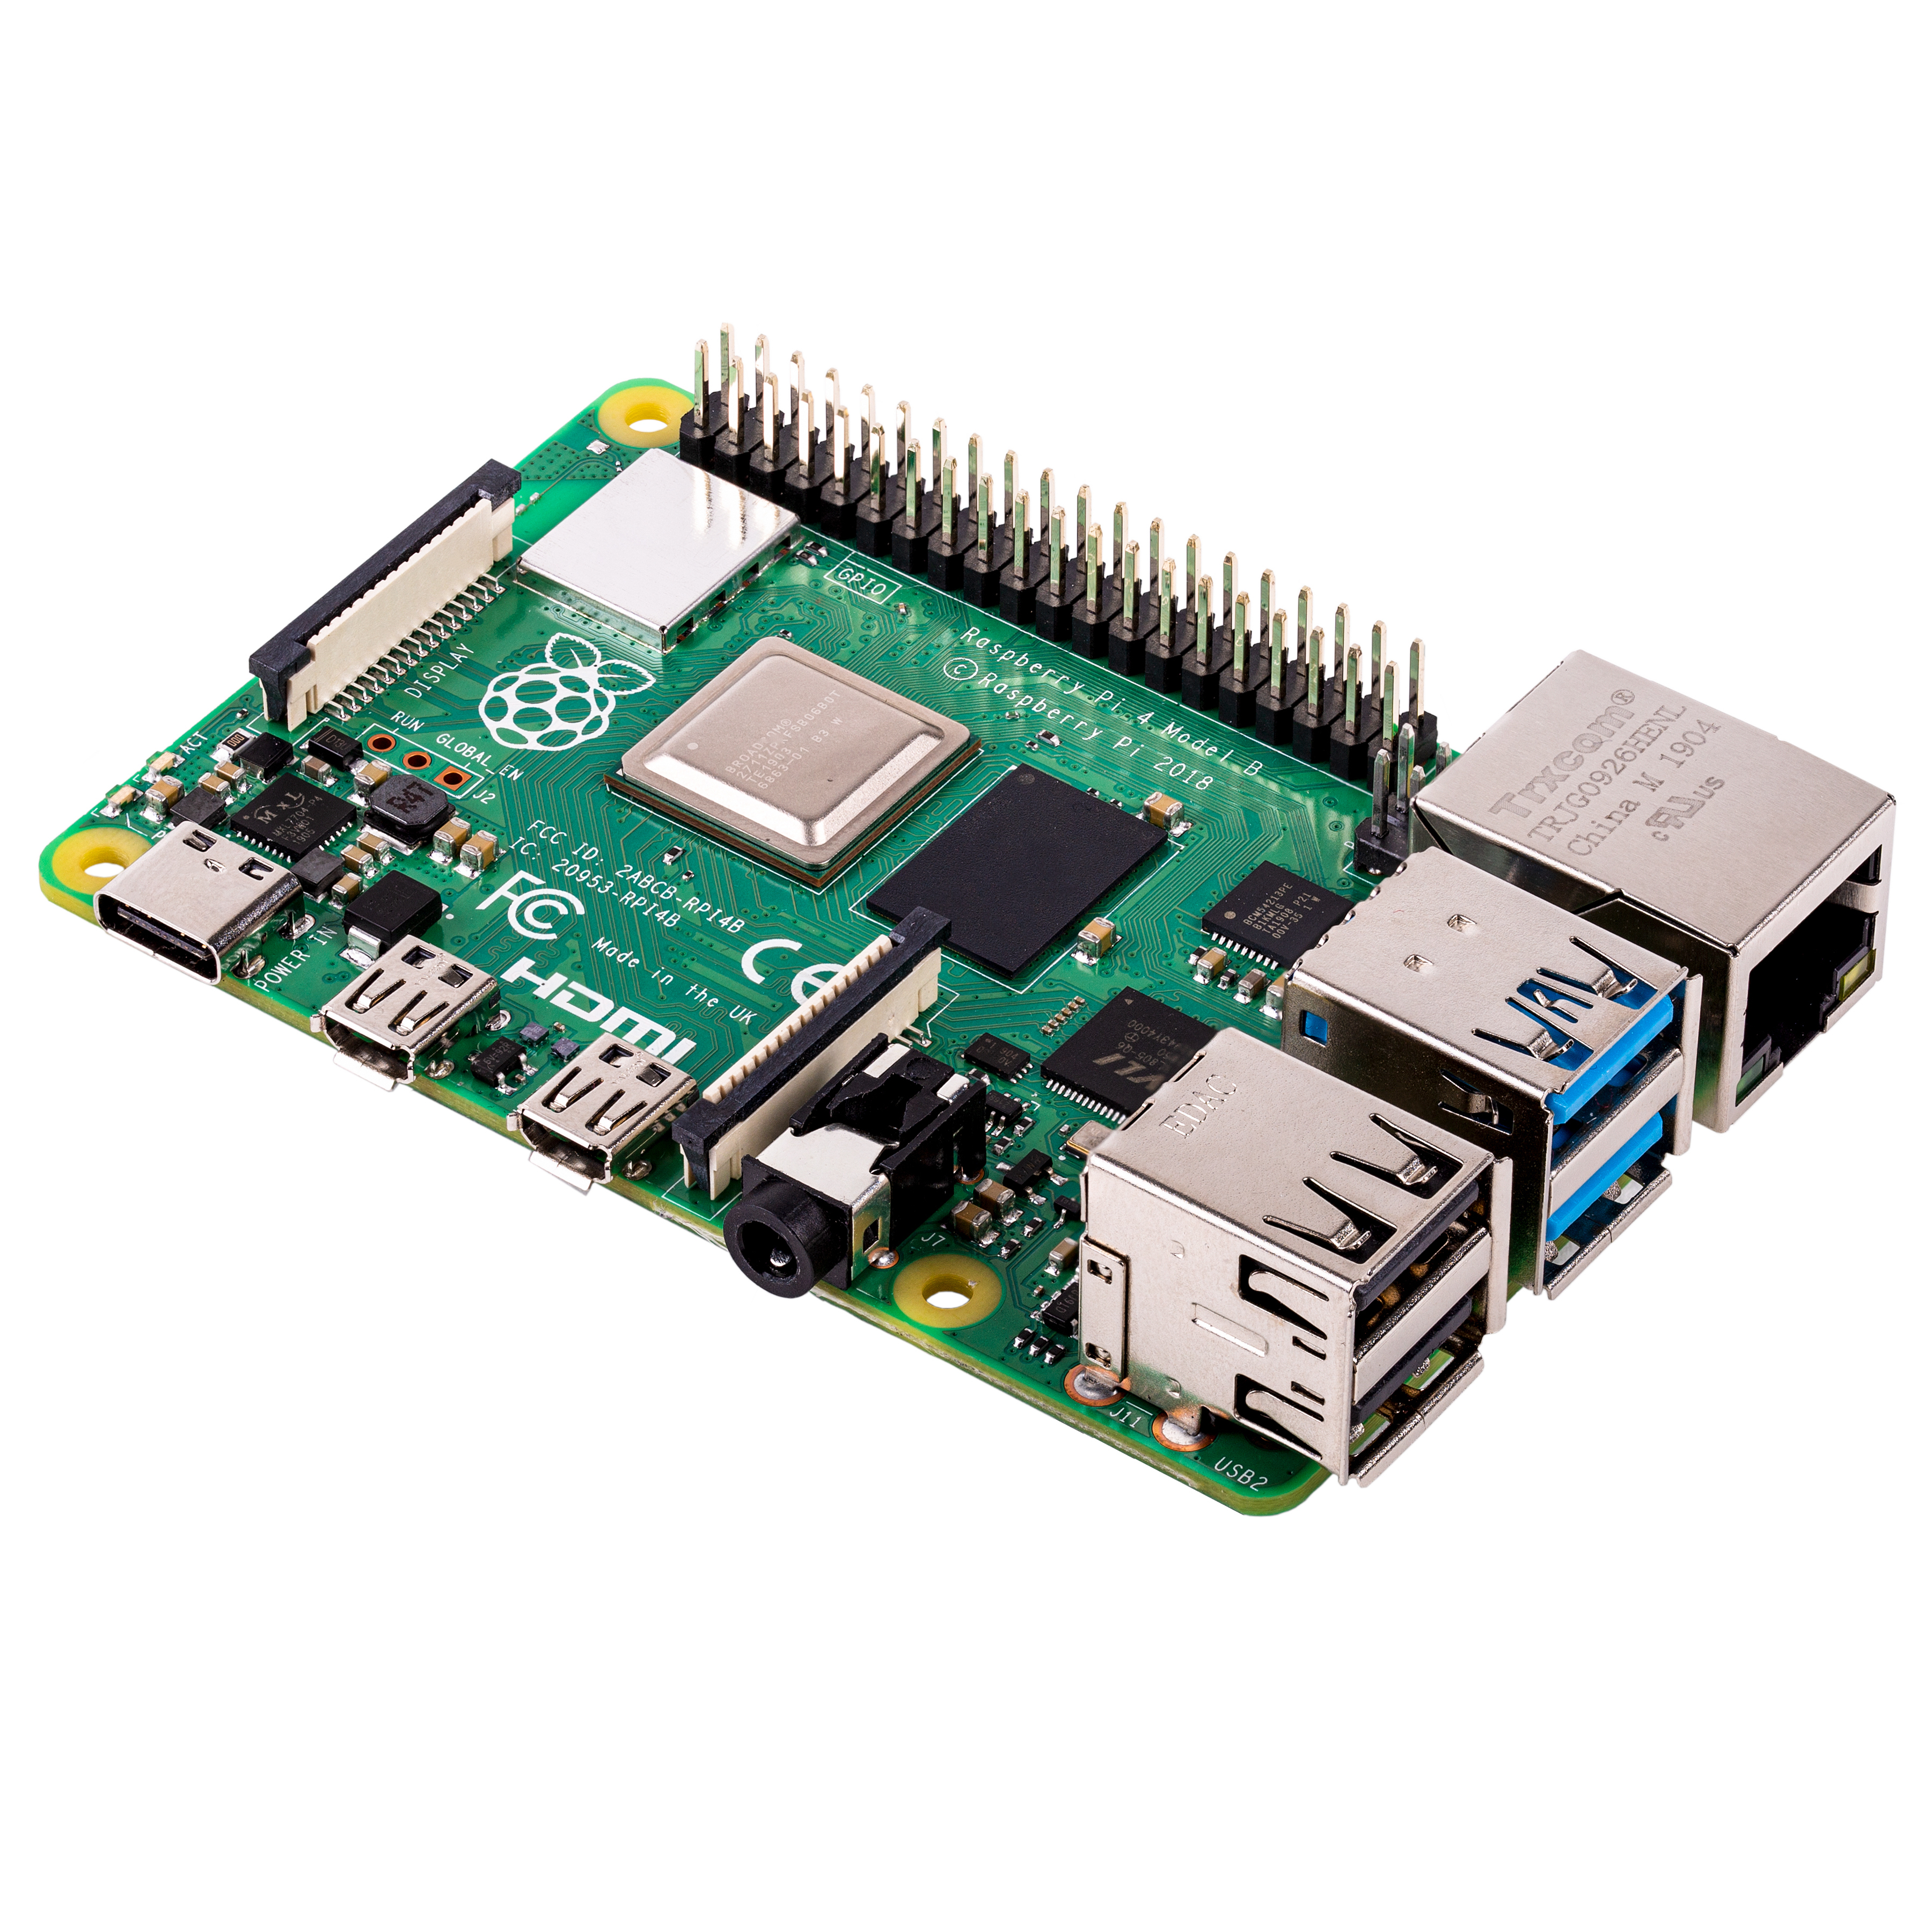
\includegraphics[width=0.5\textwidth]{images/raspberrypi.jpg}
    \caption{Raspberry Pi 4 Model B used in PiIrrigate}
    \label{fig:raspberrypi}
\end{figure}

\section{Hardware Architecture}
The hardware architecture of the PiIrrigate system consists 
of multiple ESP32 nodes that collect data from the sensors and send it to a gateway ESP32 connected to a Raspberry Pi.
The Raspberry Pi acts as a gateway that receives data from the ESP32 nodes and sends it to Azure IoT Hub using MQTT protocol.
The ESP32 nodes are connected to various sensors that collect data from the environment.

The ESP32 nodes are connected to the sensors and actuators as follows:
\begin{itemize}
  \item Soil moisture (YL-69) sensor is connected to GPIO32.
  \item Temperature and humidity sensor (DHT11) is connected to GPIO27.
  \item Rain sensor (YL-83) is connected to GPIO32.
  \item Water flow sensor {YF-S201} is connected to GPIO35.
  \item Water temperature sensor (DS18B20) is connected to GPIO26.
  \item The relay module that controls the electronic valve is connected to GPIO22.
\end{itemize}

In the figure below, you can see a simplified digram of the ESP32 pinout and connections.

\begin{figure}[H]
    \centering
    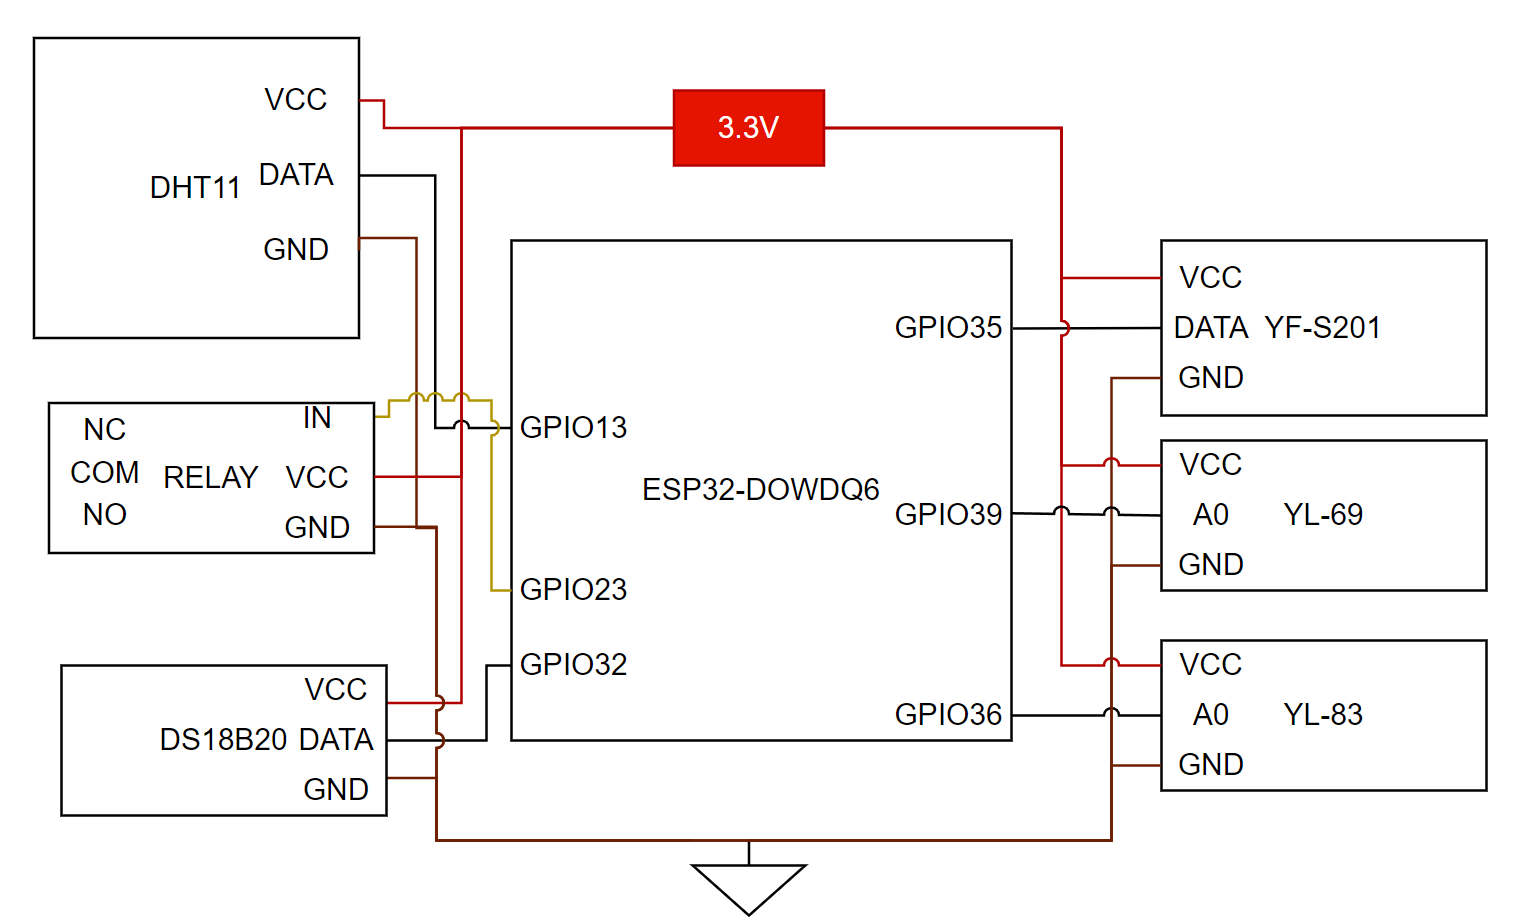
\includegraphics[width=0.8\textwidth]{images/esp-diagram.png}
    \caption{ESP32 pinout and connections}
    \label{fig:esp32-pinout}
\end{figure}

The communication between the gateway ESP32 and the Raspberry Pi is done using UART (Universal Asynchronous Receiver-Transmitter) protocol.
The gateway ESP32 receives data from the nodes using LoRa radio communication and sends it to the Raspberry Pi using UART.
In the figure below it is described the connection between the ESP32 and the Raspberry Pi.

\begin{figure}[H]
    \centering
    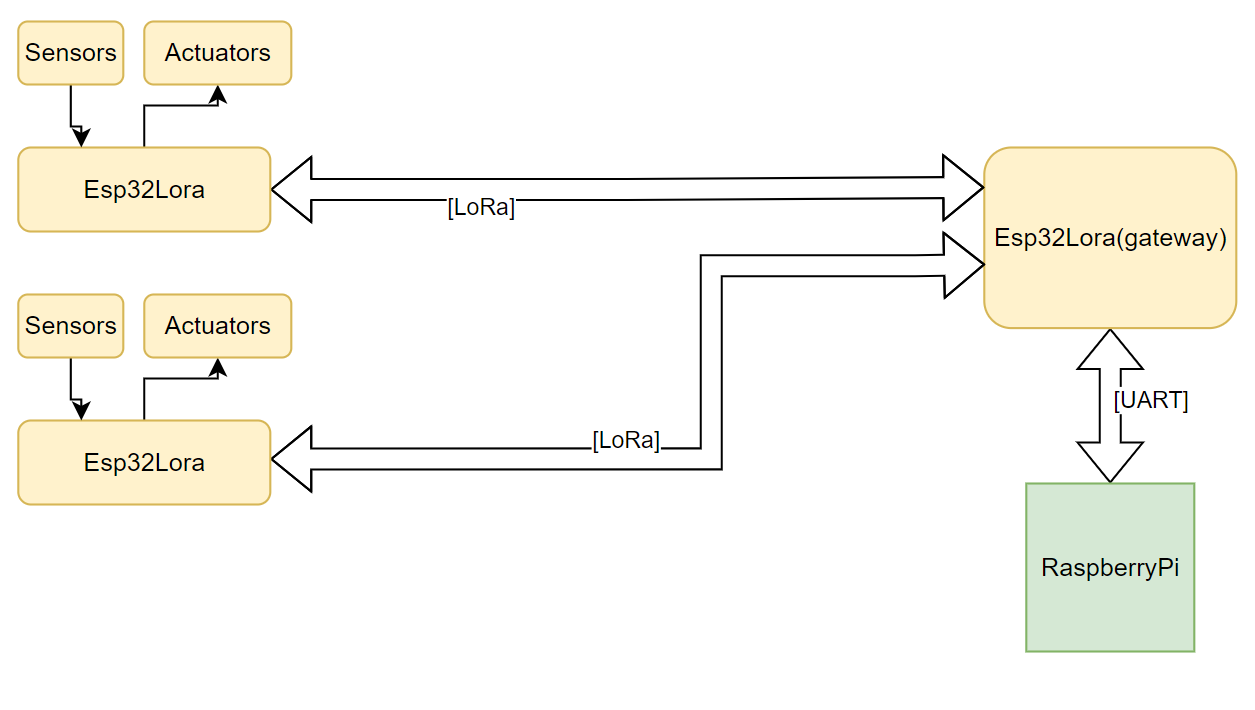
\includegraphics[width=0.8\textwidth]{images/hardware-architecture.png}
    \caption{ESP32 Gateway connection to Raspberry Pi}
    \label{fig:esp32-gateway}
\end{figure}

\section{Software Components}
PiIrrigate system contains multiple software components that work together to provide a complete solution.
The main sofware components of the PiIrrigate system are: ESP32 firmware, Raspberry Pi script, 
Web API together with the PostgreSQL database, and Web Application.

\section {Software Architecture}
The software architecture of the PiIrrigate system is a headless architecure. Headless architecture is a software development
approache that separates the frontend and backend of an application, allowing for faster development and better 
customization \cite{headlessArchitecture}.

Excluding the necessary code for the firmware running on the ESP32 nodes and the python script
running on the RaspberryPi, the code can be divided into 2 main components: Frontend and Backend. 
Both backend and frontend architectures are layer based, with each layer having a specific role in the system.
The backend is divided into 5 layers: Api, Service, Data, Models and Integration.

The Api layer is responsible for exposing endpoints, handling HTTP requests, performing input validation, and 
returning responses to the client. It represents the entry point of the backend application\cite{layerArchitecture}.
The service layer is the one that contains the bussiness logic of the application and 
is responsible for processing the data received from the Data layer and returning it to the Api layer.
Data layer's only role is to interact with the database. It is responsible for data access and persistence and it 
is the only layer that interacts with the database as any other layer should not be aware of the database
and should interact with the database only through the Data layer. Models layer
is responsible for defining the data structures used in the application.
The integration layer is responsible for integrating with external services, such as Azure IoT Hub and SignalR.

The frontend is also divided into 5 layers: Presenation, State, Services, Models and Guards. The Presentation layer 
is responsible for rendering the user interface and handling user interactions. The State layers is responsible for
storing the application state and managin the data flow between the components \cite{ngrxStoreGuide}. 
Service layers is responsible for interacting with the backend API and provifing ready to use data to the Presentation layer.
Models layer, similar to the backend Models layer is responsible for defining the data structures used in the application\cite{typescriptInterfaces}.
Routing layer manages the navigation between different components\cite{angularServices} and the Guards layer makes sure that the user
has the necessary permissions to access a specific route or component\cite{angularGuards}. 
In the following figure, you can see the sofware architecure of the PiIrrigate system.
\begin{figure}[H]
    \centering
    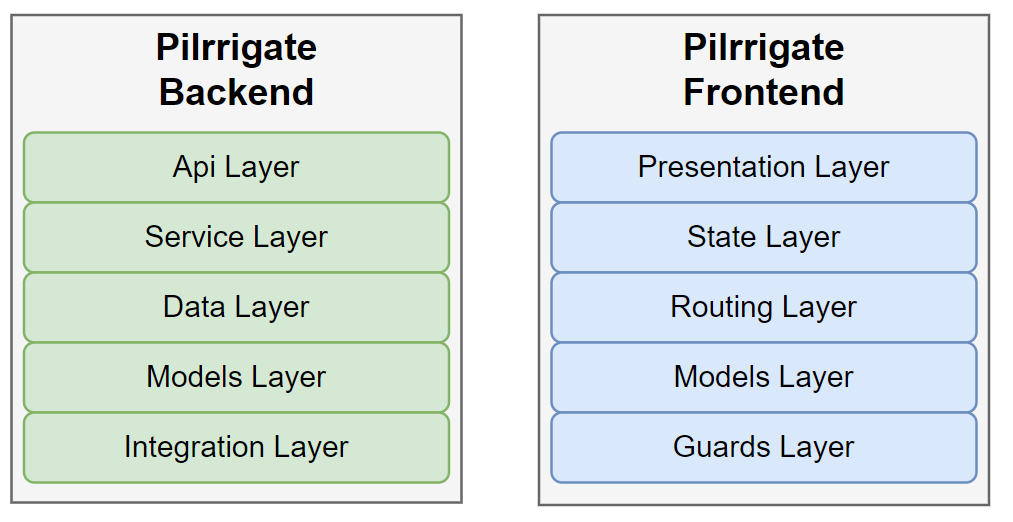
\includegraphics[width=0.5\textwidth]{images/sw-architecture.png}
    \caption{PiIrrigate Software Architecture}
    \label{fig:software-architecture}
\end{figure}

\section{Data Flow}
The data flow in the PiIrrigate system is as follows:
Data is collected from the sensors connected to the ESP32 nodes. Then the data is sent to the gateway via LoRa radio communication.
The gateway transmits the data to the Raspberry Pi using UART protocol and the Raspberry Pi send the data to Azure Iot Hub
using MQTT protocol. The Web API receives the data from the Azure IoT Hub and stores in the PostgreSQL database and
send the data to the web application using SignalR. Then the web application displays the data to the end user 
in real-time.
The data flow is illustrated in the figure below:
\begin{figure}[H]
    \centering
    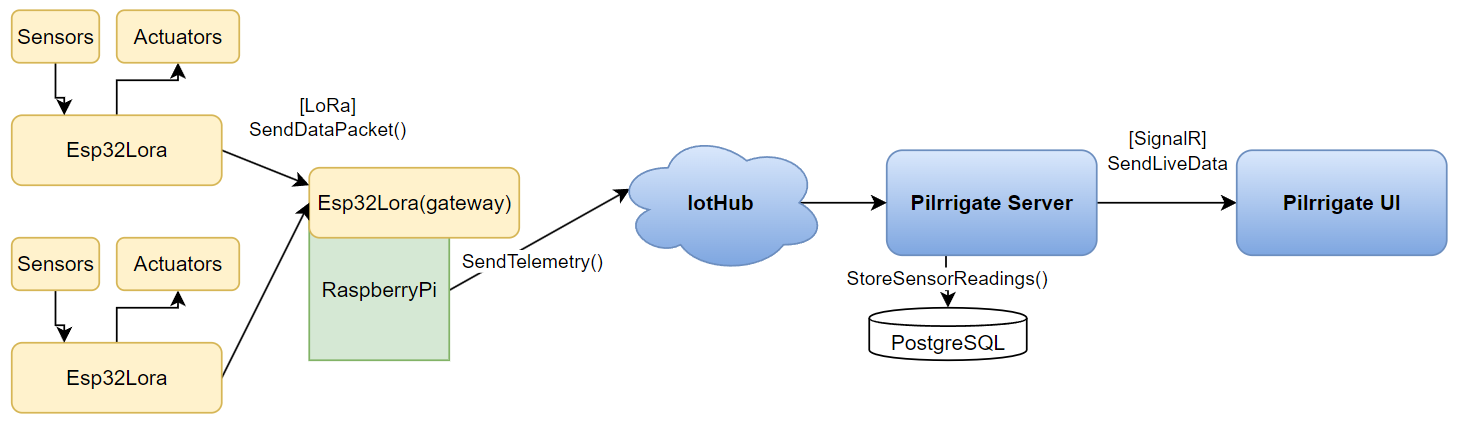
\includegraphics[width=0.8\textwidth]{images/data-flow.png}
    \caption{PiIrrigate System overview}
    \label{fig:system-overview}
\end{figure}

